\documentclass{article}
\usepackage{graphicx}
\usepackage{float}
\title{chapter 2: 2.9.2 Programming assignments}
\author{Nan Ziqian
    \and 3210104676}
\date{\today}


\begin{document}
\maketitle
\section{B}

    
    \begin{figure}[H]
        \centering
        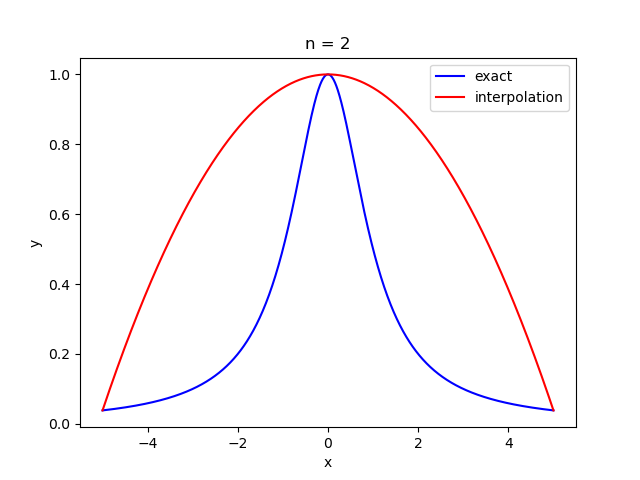
\includegraphics{../code/output/B_n2.png}
        \caption{n=2}
    \end{figure} 

    \begin{figure}[H]
        \centering
        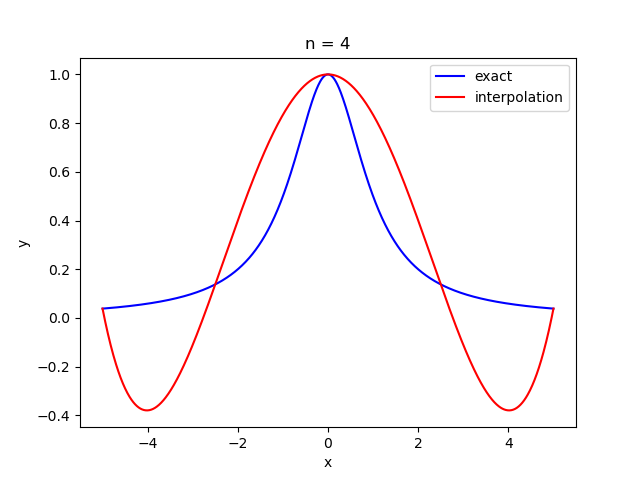
\includegraphics{../code/output/B_n4.png}
        \caption{n=4}
    \end{figure} 

    \begin{figure}[H]
        \centering
        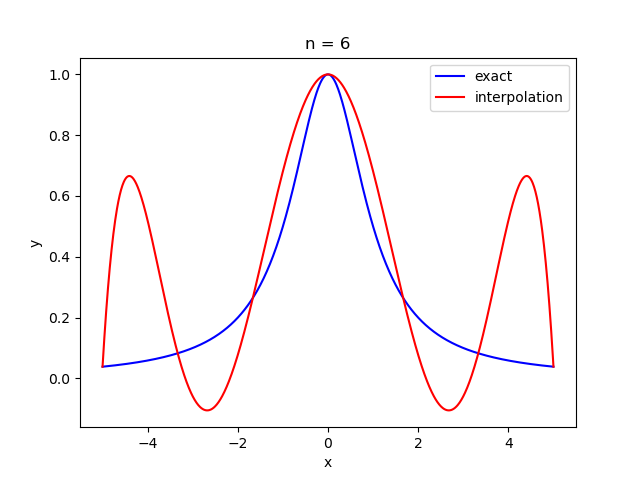
\includegraphics{../code/output/B_n6.png}
        \caption{n=6}
    \end{figure} 

    \begin{figure}[H]
        \centering
        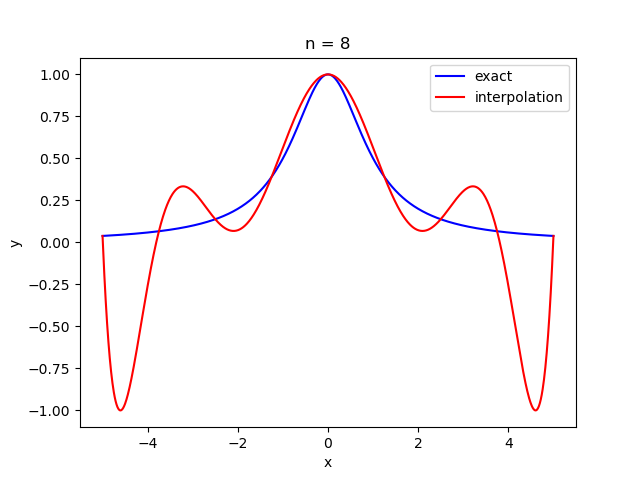
\includegraphics{../code/output/B_n8.png}
        \caption{n=8}
    \end{figure} 

\section{C}

    \begin{figure}[H]
        \centering
        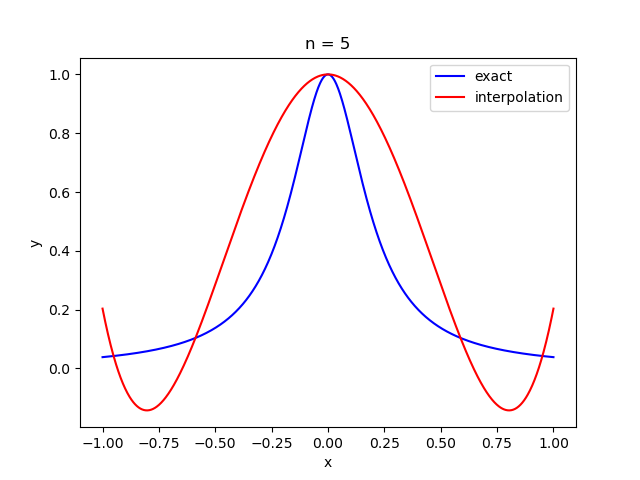
\includegraphics{../code/output/C_n5.png}
        \caption{n=5}
    \end{figure} 

    \begin{figure}[H]
        \centering
        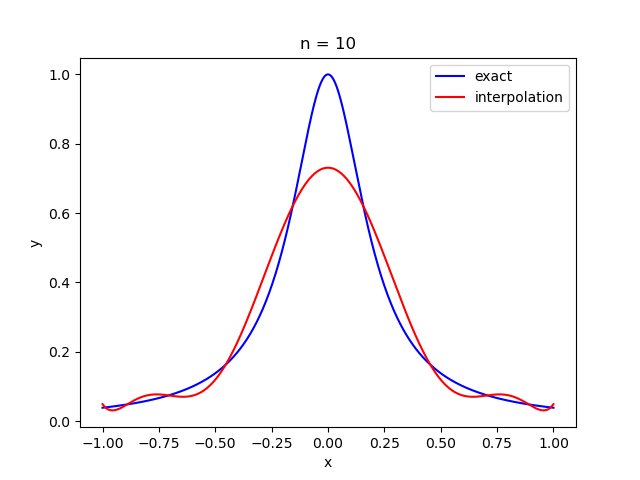
\includegraphics{../code/output/C_n10.png}
        \caption{n=10}
    \end{figure} 

    \begin{figure}[H]
        \centering
        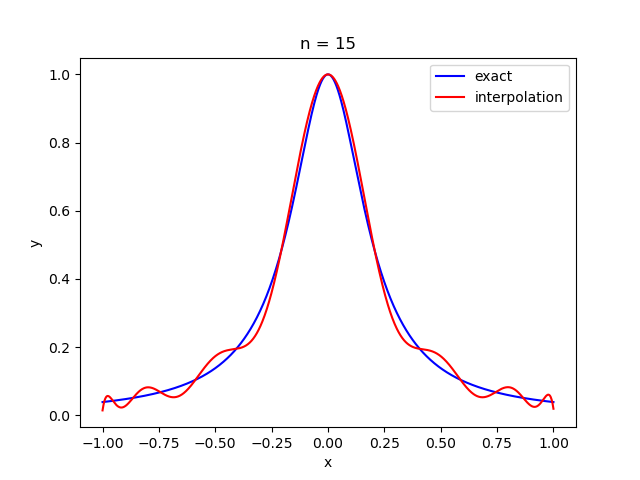
\includegraphics{../code/output/C_n15.png}
        \caption{n=15}
    \end{figure} 

    \begin{figure}[H]
        \centering
        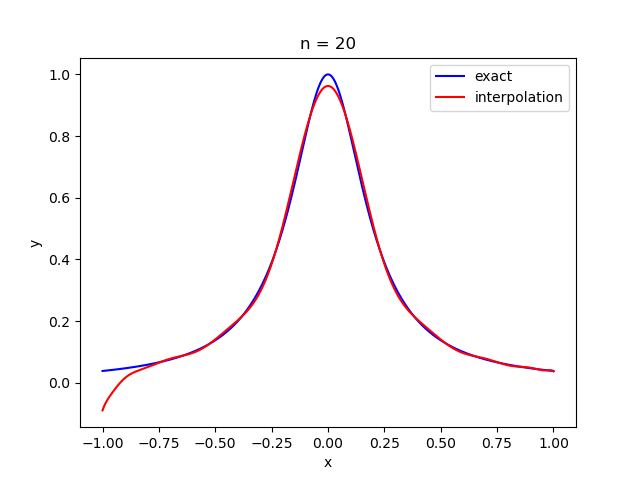
\includegraphics{../code/output/C_n20.png}
        \caption{n=20}
    \end{figure} 

\section{D}
    \subsection{(a)}
    
    The velocity of the car at t=10 is 48.3775 m/s.

    \subsection{(b)}
    The car's speed exceeds 81 m/s between t = 5.92092 and t = 6.94895
    
    The car's speed exceeds 81 m/s between t = 11.3734 and t = 12.9479

\section{E}
    \begin{figure}[H]
        \centering
        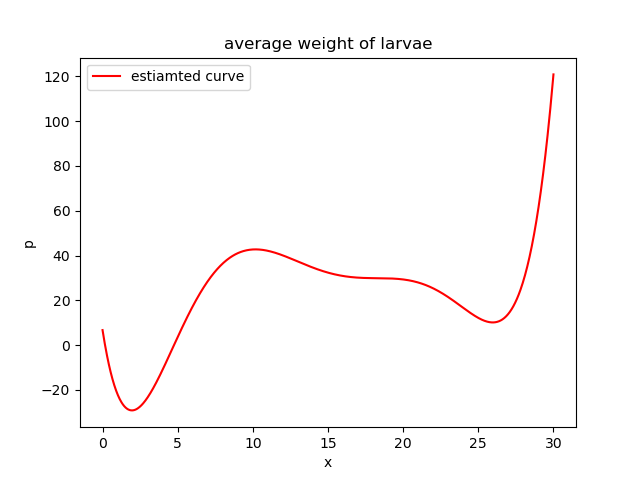
\includegraphics{../code/output/E_0.png}
        \caption{young tree}
    \end{figure} 

    \begin{figure}[H]
        \centering
        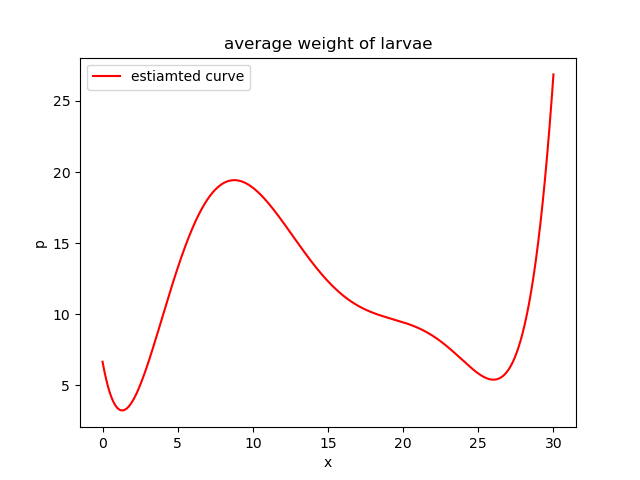
\includegraphics{../code/output/E_1.png}
        \caption{old tree}
    \end{figure}

    As we can see from the graphs the weight of larvae exploded because of the Runge phenomenon,
    so we can't accurately predict the weight of larvae in the future.

\end{document}
